\documentclass[10pt,a4paper]{article}
\usepackage[margin=2.2cm,top=2.4cm,headsep=0.5cm]{geometry}
\usepackage[T1]{fontenc}
\usepackage{lmodern}
\usepackage[scaled=0.94]{helvet}
\renewcommand{\familydefault}{\sfdefault}
\usepackage{microtype}
\usepackage[parfill]{parskip}
\usepackage{fancyhdr}
\usepackage{titlesec}
\usepackage{amsmath,amssymb}
\usepackage{graphicx}
\usepackage{booktabs}
\usepackage{array}
\usepackage{caption}
\usepackage{algorithm}
\usepackage{algpseudocode}
\usepackage[dvipsnames]{xcolor}
\usepackage{listings}
\usepackage[colorlinks=true,linkcolor=MidnightBlue,citecolor=MidnightBlue,urlcolor=MidnightBlue]{hyperref}
\usepackage[nameinlink]{cleveref}

\graphicspath{{../figures/}}
% generated by scripts/make_plots.py -- do not edit
\newcommand{\CGbwAll}{1299}
\newcommand{\CGbwFrac}{77}
\newcommand{\CGbwNode}{215}
\newcommand{\CGbwOne}{23.9}
\newcommand{\CGbwPerNodeMax}{162}
\newcommand{\CGbwTB}{1.30}
\newcommand{\CVN}{256}
\newcommand{\CVP}{64}
\newcommand{\CVmsgsOneD}{2}
\newcommand{\CVmsgsThreeD}{6}
\newcommand{\CVoneD}{1.00}
\newcommand{\CVratio}{5.3}
\newcommand{\CVthreeD}{0.19}
\newcommand{\CommFracNode}{5}
\newcommand{\CommFracPmax}{40}
\newcommand{\EffFour}{98}
\newcommand{\EffNode}{28}
\newcommand{\EffPmax}{22}
\newcommand{\FinalCG}{$6\times10^{-13}$}
\newcommand{\FinalPipe}{$4\times10^{-9}$}
\newcommand{\FloorCG}{$6\times10^{-13}$}
\newcommand{\FloorPipe}{$1\times10^{-11}$}
\newcommand{\FloorRatio}{15}
\newcommand{\GpuBwFiveTwelve}{473}
\newcommand{\GpuBwFrac}{68}
\newcommand{\GpuBwMax}{474}
\newcommand{\GpuBwMin}{416}
\newcommand{\GpuCGoneRel}{2}
\newcommand{\GpuDofsMax}{453}
\newcommand{\GpuDriver}{575.57.08}
\newcommand{\GpuMLUPS}{5.37}
\newcommand{\GpuMem}{45}
\newcommand{\GpuModule}{nvhpc-hpcx-cuda12/26.1}
\newcommand{\GpuNVC}{26.1-0}
\newcommand{\GpuName}{NVIDIA A40}
\newcommand{\GpuNmax}{768}
\newcommand{\GpuNmin}{128}
\newcommand{\GpuSpmvBw}{415}
\newcommand{\GpuSpmvFrac}{31}
\newcommand{\GpuTfiveTwelve}{25.0}
\newcommand{\GpuValFail}{0}
\newcommand{\GpuValP}{1, 2, 4, 8}
\newcommand{\GpuValRuns}{8}
\newcommand{\GpuValWorst}{$4.0\times10^{-15}$}
\newcommand{\GpuVecBw}{499}
\newcommand{\GpuVsCore}{22}
\newcommand{\GpuVsEight}{2.5}
\newcommand{\GpuVsSocket}{2.4}
\newcommand{\HaloFracPmax}{11}
\newcommand{\HaloKiBNode}{1152}
\newcommand{\HaloKiBPmax}{320}
\newcommand{\HaloMsPmax}{1.12}
\newcommand{\HybBest}{32$\times$8}
\newcommand{\HybBestT}{8.72}
\newcommand{\HybCores}{256}
\newcommand{\HybGain}{6}
\newcommand{\HybPureT}{9.23}
\newcommand{\HybRange}{9}
\newcommand{\HybRedBest}{1.51}
\newcommand{\HybRedPure}{2.07}
\newcommand{\HybWorst}{8$\times$32}
\newcommand{\HybWorstT}{9.46}
\newcommand{\Iters}{50}
\newcommand{\LastCG}{365}
\newcommand{\LastPipe}{700}
\newcommand{\MachineCPN}{32}
\newcommand{\MachineCPS}{36}
\newcommand{\MachineCPU}{Intel(R) Xeon(R) Platinum 8452Y}
\newcommand{\MachineCores}{256}
\newcommand{\MachineGCC}{13.1.0}
\newcommand{\MachineMPI}{Open MPI 4.1.8}
\newcommand{\MachineNodes}{8}
\newcommand{\MaxSpread}{166}
\newcommand{\MedSpread}{3.7}
\newcommand{\NS}{512}
\newcommand{\NSdofs}{134}
\newcommand{\NStwo}{768}
\newcommand{\NStwoDofs}{453}
\newcommand{\NodeCPU}{Intel(R) Xeon(R) Platinum 8452Y}
\newcommand{\NodeEffPmax}{76}
\newcommand{\NodeEffSixtyFour}{83}
\newcommand{\NodeEffTwoPmax}{83}
\newcommand{\NodeSpeedPmax}{6.06}
\newcommand{\NodeSpeedTwoPmax}{6.60}
\newcommand{\NodeValCG}{$3.8\times10^{-15}$}
\newcommand{\NodeValEdge}{12}
\newcommand{\NodeValPipe}{$2.0\times10^{-12}$}
\newcommand{\NodeValResult}{passes}
\newcommand{\NodeValRuns}{36}
\newcommand{\NodesMax}{8}
\newcommand{\Pmax}{256}
\newcommand{\PoneFaster}{faster}
\newcommand{\PoneTiter}{540}
\newcommand{\PoneVsSerial}{1.2}
\newcommand{\RedFracPmax}{28}
\newcommand{\RedMsNode}{1.04}
\newcommand{\RedMsPmax}{2.81}
\newcommand{\RelBlocking}{0.92}
\newcommand{\RelBlockingRange}{0.92--1.01}
\newcommand{\RelCGone}{0.95}
\newcommand{\RelCGonemin}{1.01}
\newcommand{\RelOneD}{1.53}
\newcommand{\RelOneDmin}{1.14}
\newcommand{\RelPipe}{1.15}
\newcommand{\RelPipeBlock}{1.18}
\newcommand{\RelPipeTwo}{1.28}
\newcommand{\RelPipemin}{1.32}
\newcommand{\RelTwoD}{1.06}
\newcommand{\RelTwoDRange}{0.95--1.06}
\newcommand{\Reps}{3}
\newcommand{\SerialTiter}{546}
\newcommand{\SizesCPU}{Intel(R) Xeon(R) Platinum 8452Y}
\newcommand{\SolveCG}{21.0}
\newcommand{\SolveCGTrue}{$9.8\times10^{-9}$}
\newcommand{\SolveCGone}{20.6}
\newcommand{\SolveGpu}{48.5}
\newcommand{\SolveGpuIters}{1942}
\newcommand{\SolveGpuSpeedup}{24}
\newcommand{\SolveIters}{1942}
\newcommand{\SolvePipe}{25.5}
\newcommand{\SolvePipeRatio}{70}
\newcommand{\SolvePipeTrue}{$7.0\times10^{-7}$}
\newcommand{\SolveSpeedup}{56}
\newcommand{\SpeedupEight}{5.8}
\newcommand{\SpeedupFour}{3.91}
\newcommand{\SpeedupNode}{9.1}
\newcommand{\SpeedupPmax}{55.1}
\newcommand{\SplitCG}{$2\times10^{-13}$}
\newcommand{\SplitPipe}{$3\times10^{-11}$}
\newcommand{\StreamAll}{279}
\newcommand{\StreamEight}{131}
\newcommand{\StreamOne}{20.0}
\newcommand{\StreamThreads}{32}
\newcommand{\SzBwLarge}{21.1}
\newcommand{\SzBwMax}{30}
\newcommand{\SzBwMin}{17}
\newcommand{\SzItMax}{1942}
\newcommand{\SzItMin}{235}
\newcommand{\SzItPerN}{3.79}
\newcommand{\SzNmax}{512}
\newcommand{\SzNmin}{64}
\newcommand{\SzNsLarge}{4.55}
\newcommand{\SzNsMax}{5.62}
\newcommand{\SzNsMin}{3.21}
\newcommand{\SzNsSmall}{4.13}
\newcommand{\SzRuns}{9}
\newcommand{\SzSlopeIter}{3.05}
\newcommand{\SzSlopeSolve}{4.06}
\newcommand{\SzSolveMax}{1187}
\newcommand{\SzSolveMaxMin}{19.8}
\newcommand{\SzSolveMin}{0.25}
\newcommand{\SzTiterMax}{611}
\newcommand{\TiterNode}{60.1}
\newcommand{\TiterPmax}{9.92}
\newcommand{\TiterSixtyFour}{36.0}
\newcommand{\TiterTwoNode}{201.6}
\newcommand{\TiterTwoPmax}{30.5}
\newcommand{\ValEdge}{30}
\newcommand{\ValErrMax}{$2.39\times10^{-5}$}
\newcommand{\ValIters}{146}
\newcommand{\ValN}{40}
\newcommand{\ValRuns}{180}
\newcommand{\ValWorstCG}{$3.8\times10^{-15}$}
\newcommand{\ValWorstPipe}{$2.0\times10^{-12}$}
\newcommand{\VarP}{256}
\newcommand{\VarPmin}{32}
\newcommand{\VecFracSerial}{56}
\newcommand{\WeakBwNode}{6.8}
\newcommand{\WeakBwOne}{18.1}
\newcommand{\WeakDofsMax}{1.81}
\newcommand{\WeakEffNode}{38}
\newcommand{\WeakEffPmax}{30}
\newcommand{\WeakLocal}{192}
\newcommand{\WeakNmax}{1219}
\newcommand{\WeakNodeEff}{80}
\newcommand{\WeakPmax}{256}
\newcommand{\WeakTmax}{125.1}
\newcommand{\WeakTnode}{100.5}
\newcommand{\WeakTone}{37.4}


% \input inside a tabular breaks \bottomrule; the TeX primitive does not
\makeatletter\newcommand{\tabinput}[1]{\@@input #1 }\makeatother
\captionsetup{font=normalsize,labelfont=normalfont,labelsep=colon,skip=6pt}
\titleformat{\section}{\large\bfseries}{\thesection.}{0.5em}{}
\titleformat{\subsection}{\normalsize\bfseries}{\thesubsection}{0.6em}{}
\titlespacing*{\section}{0pt}{14pt}{6pt}
\titlespacing*{\subsection}{0pt}{10pt}{4pt}
\pagestyle{fancy}\fancyhf{}
\fancyhead[L]{\small DSA5208 \textbar{} Parallel Conjugate Gradients}
\fancyhead[R]{\small MPI\,+\,OpenMP on NUS Vanda}
\fancyfoot[C]{\small\thepage}
\renewcommand{\headrulewidth}{0.4pt}
\lstset{basicstyle=\ttfamily\small,columns=fullflexible,keepspaces=true,frame=single,
        framerule=0.3pt,rulecolor=\color{gray!60},backgroundcolor=\color{gray!4}}
\newcommand{\code}[1]{\texttt{#1}}
\newcommand{\vb}[1]{\mathbf{#1}}
\emergencystretch=2em

\begin{document}
\thispagestyle{plain}
\begin{center}
{\LARGE\bfseries Scaling Conjugate Gradients with MPI and OpenMP\par}
\vspace{4pt}
{\large Decomposition, communication hiding and memory bandwidth in a matrix-free 3D Poisson solver\par}
\vspace{10pt}
\begin{tabular*}{\linewidth}{@{\extracolsep{\fill}}ccc}
WU YUHAN (A0351706H) & ZUO DEWEI (A0352507H) & ZHU CHEN (A0357394N)
\end{tabular*}\par
\vspace{6pt}
DSA5208 $\cdot$ Project 3\par
\end{center}
\vspace{4pt}

\noindent{\large\bfseries Abstract}\par
\noindent
The Conjugate Gradient (CG) method is the standard solver for the symmetric positive definite systems
produced by elliptic partial differential equations, and it is notoriously hard to scale: every iteration
needs a nearest-neighbour exchange, two global reductions and a full sweep through memory. We build a
matrix-free hybrid MPI\,+\,OpenMP CG solver for the 3D Poisson equation in which the four central
parallelisation decisions---domain decomposition, halo exchange, reduction strategy and the split between
processes and threads---are run-time switches, and measure each of them on the NUS Vanda cluster. The solver
reproduces the serial solution to \ValWorstCG{} in \ValRuns{} parallel configurations and converges at the
theoretical second order. On 36 cores of a Vanda node it reaches a speedup of \SpeedupPmax{} on a $512^3$
grid and sustains \CGbwAll\,GB/s, 70\% of the node's STREAM bandwidth: inside a node, CG scales exactly as
far as memory bandwidth does. A memory-traffic model predicts the design trade-offs: pipelined CG pays its
36\% traffic surcharge almost in full (\RelPipe$\times$ measured) and leaves its true residual
\SolvePipeRatio{} times above the tolerance, slabs fall 13\% behind blocks, overlapped halos only pay across a
network, and the global reductions act mainly as barriers that turn bandwidth imbalance into waiting.

\section{Introduction}\label{sec:intro}

Many simulation codes spend most of their run time solving a single kind of linear system. The pressure
projection of incompressible flow solvers, the electrostatic potential in plasma and molecular dynamics,
the gravitational potential in astrophysics and graph-Laplacian systems in semi-supervised learning and
spectral clustering all reduce to a Poisson-type equation that has to be solved again at every time step
or outer iteration. Discretising $-\nabla^2u=f$ on a cube with $N$ grid points per direction yields
$N^3$ unknowns, and refining the grid makes the problem harder twice over: the system grows like $N^3$,
and the number of iterations of a Krylov solver grows like $N$, so the total work grows like $N^4$. A
$512^3$ grid already holds 134 million unknowns and needs about two thousand CG iterations. Solving such
problems in reasonable time and memory requires distributing them across many nodes.

The Conjugate Gradient method is the method of choice for these symmetric positive definite systems, and
it is also a standard stress test for parallel computers: the HPCG benchmark, which complements LINPACK
in the TOP500 ranking, is built around it because supercomputers reach only a few percent of their peak
performance on it. The reason lies in the structure of a single iteration. Its matrix--vector product
couples every unknown to its grid neighbours, so a distributed implementation has to exchange the
boundary layers (\emph{halos}) of every subdomain in every iteration. Its two inner products couple every
unknown to every other one; each requires a global reduction that acts as a barrier across all
processes and whose latency grows with the number of processes $P$. Since every iteration needs the
scalars produced by the previous one, none of this communication can be batched or deferred across
iterations. What remains after communication---the stencil and the vector updates---performs about
17 floating-point operations per 88 bytes of memory traffic, so even the perfectly parallel local work is
limited by the memory bandwidth that all cores of a socket share.

Each of these obstacles admits several engineering answers, and the answers interact. A
three-dimensional block decomposition minimises the halo volume but sends more, smaller and strided
messages than a slab decomposition. Non-blocking communication can hide the halo exchange behind interior
computation, but only if the MPI library actually progresses the messages and the deferred boundary work
does not destroy cache locality. Algebraic reformulations of CG merge the two reductions into one or
overlap the reduction with the matrix--vector product, at the price of extra vectors, extra memory
traffic and weaker numerical stability. OpenMP threads inside each MPI process cut the number of messages
and of reduction participants, at the price of fork--join overhead and threads that idle while the master
thread communicates.

This project implements a serial reference solver and a hybrid MPI\,+\,OpenMP solver in C in which each of
these choices is a run-time switch, so that its effect is measured in isolation on an identical problem.
We validate the parallel solver point by point against the serial one in \ValRuns{} configurations and
against an analytical solution, derive a performance model from memory traffic and communication volume,
and instrument the solver with per-phase timers and byte counters that explain the measured scaling
rather than merely report it. \Cref{sec:algorithm} introduces the problem and the algorithm,
\cref{sec:design} develops the parallel design and the performance model, \cref{sec:validation} validates
the implementation and \cref{sec:perf} analyses its performance.

\section{The model problem and the Conjugate Gradient method}\label{sec:algorithm}

We solve the Poisson equation $-\nabla^2 u = f$ on the unit cube $\Omega=(0,1)^3$ for an unknown
function $u:\Omega\to\mathbb{R}$ and a given source $f$, with the homogeneous Dirichlet condition $u=0$ on
the boundary $\partial\Omega$. A uniform grid with $N$ interior points per direction has spacing
$h=1/(N+1)$ and grid points $(x_i,y_j,z_k)=(ih,jh,kh)$ for $i,j,k\in\{1,\dots,N\}$; we write $u_{ijk}$ for
the approximation of $u(x_i,y_j,z_k)$. Replacing each second derivative by the centred difference
$(u_{i-1}-2u_i+u_{i+1})/h^2$ and multiplying by $h^2$ gives the linear system $A\vb u=\vb b$ with
\begin{equation}\label{eq:stencil}
\begin{aligned}
  (A\vb u)_{ijk} &= 6u_{ijk}-u_{i-1,j,k}-u_{i+1,j,k}-u_{i,j-1,k}-u_{i,j+1,k}-u_{i,j,k-1}-u_{i,j,k+1},\\
  b_{ijk} &= h^2 f(x_i,y_j,z_k),
\end{aligned}
\end{equation}
where values with an index equal to $0$ or $N+1$ are boundary values and therefore zero. The matrix
$A\in\mathbb{R}^{N^3\times N^3}$ is symmetric positive definite with condition number
$\kappa(A)\approx 4/(\pi^2h^2)$. We never assemble $A$: it is applied as the 7-point stencil
\eqref{eq:stencil} (\emph{matrix-free}), so memory consumption and memory traffic are entirely those of
the vectors.

To test the solver we prescribe the exact solution $u(x,y,z)=g(x)\,g(y)\,g(z)$ with $g(t)=t(1-t)e^{t}$,
which vanishes on $\partial\Omega$, and compute the matching source $f=-\nabla^2 u$ analytically using
$g''(t)=-t(3+t)e^t$. The common choice $\sin(\pi x)\sin(\pi y)\sin(\pi z)$ would be useless here: it is
an eigenvector of the discrete operator, CG converges on it in a single iteration, and the test would
hide most bugs. For our $u$ the discrete solution differs from the exact one by a genuine $O(h^2)$ error,
which turns the comparison with $u$ into a sharp end-to-end test.

CG (\cref{alg:cg}) builds the iterates $\vb x_k$ from the residuals $\vb r_k=\vb b-A\vb x_k$ and the
search directions $\vb p_k$; the step length $\alpha_k$ minimises the $A$-norm of the error along
$\vb p_k$, and $\beta_{k+1}$ keeps the new direction $A$-conjugate to all previous ones. The scalar
$\gamma_k=\|\vb r_k\|^2$ doubles as the stopping criterion with relative tolerance $\varepsilon$. The
error contracts by roughly $(\sqrt{\kappa}-1)/(\sqrt{\kappa}+1)$ per iteration, so the number of
iterations to reach a fixed $\varepsilon$ grows like $\sqrt{\kappa}\propto 1/h\propto N$. Our runs
confirm this: \ValIters{} iterations for $N=\ValN$ and \SolveIters{} for $N=\NS$ at $\varepsilon=10^{-8}$,
close to the ratio of the grid sizes. One iteration consists of one stencil application, two inner products
and three vector updates. Per grid point the stencil costs 7 floating-point operations, its inner product 2
and the updates 8, i.e.\ 17 flops, against 11 loads and stores of 8-byte values (88 bytes, see
\cref{sec:model}). At 0.2 flop/byte this is an order of magnitude below the balance of current server
processors, so CG runs at the speed of memory, not of arithmetic.

\begin{algorithm}[htb]
\caption{Conjugate Gradients for $A\vb x=\vb b$ with $\vb x_0=0$. Framed comments mark the points where a
parallel implementation must communicate.}\label{alg:cg}
\begin{algorithmic}[1]
\State $\vb r_0=\vb b,\quad \vb p_0=\vb r_0,\quad \gamma_0=\vb r_0^T\vb r_0$
\For{$k=0,1,2,\dots$ \textbf{until} $\sqrt{\gamma_k}\le \varepsilon\,\|\vb b\|$}
  \State $\vb q_k = A\vb p_k$ \Comment{\fbox{halo exchange} of $\vb p_k$, then stencil}
  \State $\alpha_k = \gamma_k/(\vb p_k^T\vb q_k)$ \Comment{\fbox{global reduction}}
  \State $\vb x_{k+1}=\vb x_k+\alpha_k\vb p_k,\ \ \vb r_{k+1}=\vb r_k-\alpha_k\vb q_k,\ \ \gamma_{k+1}=\vb r_{k+1}^T\vb r_{k+1}$ \Comment{\fbox{global reduction}}
  \State $\beta_{k+1}=\gamma_{k+1}/\gamma_k,\quad \vb p_{k+1}=\vb r_{k+1}+\beta_{k+1}\vb p_k$
\EndFor
\end{algorithmic}
\end{algorithm}

\section{Parallel design}\label{sec:design}

The parallel solver distributes the grid over $P$ MPI processes and runs $T$ OpenMP threads inside each.
This section follows the data through one iteration: how the grid is partitioned, how boundary values
travel between processes, how the global reductions are organised and how the threads share the local
work. It closes with a cost model that ties these decisions together.

\subsection{Data distribution}\label{sec:decomp}
The processes form a Cartesian grid $p_x\times p_y\times p_z=P$ created by \code{MPI\_Dims\_create} and
\code{MPI\_Cart\_create}. The process with coordinates $(c_x,c_y,c_z)$ owns a block of $n_x\times n_y\times
n_z$ grid points, where in each direction $n_d=\lfloor N/p_d\rfloor$, plus one for the first $N\bmod p_d$
coordinates; block sizes therefore differ by at most one plane and any $P$ works with any $N$. Each block is
stored with one ghost layer on every side, $(n_x+2)(n_y+2)(n_z+2)$ values with the $k$ index contiguous.
Ghost layers on the physical boundary permanently hold the Dirichlet zeros, so the stencil loop contains
no branches. The right-hand side is evaluated from one-dimensional tables of $g$ and $g''$, so no global
vector $\vb b$ is stored.

The switch \code{-d} selects slabs ($p_y=p_z=1$), pencils ($p_z=1$) or blocks (all three factors free).
The choice sets how much data each process sends per iteration. For a process in the interior of the
process grid and $N$ divisible by the factors, the number of 8-byte values sent per halo exchange is
\begin{equation}\label{eq:volume}
  V_{\text{1D}} = 2N^2,\qquad V_{\text{2D}} = \frac{4N^2}{\sqrt P},\qquad V_{\text{3D}} = \frac{6N^2}{P^{2/3}},
\end{equation}
carried by $m=2$, $4$ and $6$ messages respectively. The slab volume does not decrease with $P$, so slabs
stop scaling once the halo time becomes comparable to the computation, which shrinks like $1/P$; slabs
also cap $P$ at $N$. Blocks send the least data, but their $k$-faces consist of $n_xn_y$ values separated
by a stride of $n_z+2$, so packing them into a send buffer touches one cache line per value. The solver
counts the bytes and messages of every process, and \cref{fig:commvol} shows the measured values for
$N=\CVN$. At $P=\CVP$ the busiest process sends \CVoneD\,MiB per iteration with slabs and \CVthreeD\,MiB with
blocks, a factor of \CVratio, while the message count rises from \CVmsgsOneD{} to \CVmsgsThreeD. We use
blocks as the baseline.

\begin{figure}[t]
\centering
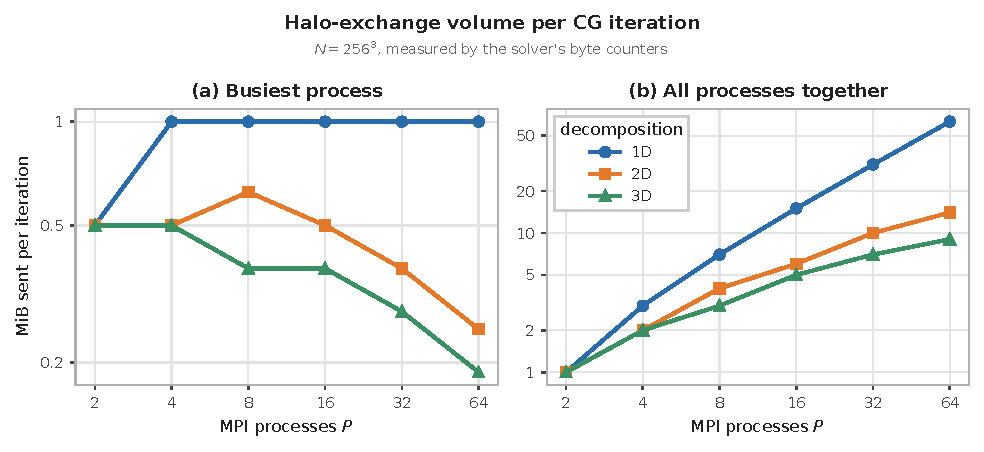
\includegraphics[width=\linewidth]{commvol}
\caption{Halo data sent per CG iteration for slab (1D), pencil (2D) and block (3D) decompositions,
$N=\CVN$, measured by the solver's counters. (a) The busiest process, which sets the exchange time on a
bandwidth-limited network; (b) the total network load.}\label{fig:commvol}
\end{figure}

\subsection{Halo exchange}\label{sec:halo}
Before each stencil application a process needs the values of the neighbouring blocks adjacent to its
faces. Because the 7-point stencil uses no edge or corner neighbours, the three directions are
independent and are exchanged together. In the \emph{blocking} mode the solver packs all six faces into
buffers within one OpenMP parallel region, performs one \code{MPI\_Sendrecv} per direction and sense,
unpacks the received faces into the ghost layers and then applies the stencil to the whole block.
Neighbours that do not exist are \code{MPI\_PROC\_NULL}, which turns the corresponding transfers into
no-ops.

The \emph{overlapped} mode exploits the fact that most points of a block do not need ghost values. It
posts \code{MPI\_Irecv} for all faces, packs, posts \code{MPI\_Isend}, applies the stencil to the interior,
waits for the messages, unpacks and finally applies the stencil to the remaining boundary shell. The shell
is covered by disjoint pieces---two $i$-planes, two $j$-rows inside them, two $k$-columns inside those---so
the fused inner product counts every point exactly once. Making this overlap effective took two further
steps. The first concerns progress: most MPI libraries, Open MPI over TCP included, move data only inside
MPI calls, and large faces use a rendezvous protocol whose handshake cannot complete while the process
computes. The solver therefore splits the interior sweep into chunks of $i$-planes (four by default) and
calls \code{MPI\_Testall} between them, which advances the transfers during the computation. The second
concerns locality. Our first version deferred the shell layers on all six sides, so with slabs every
process handled its $k=1$ and $k=n_z$ columns as isolated, strided points even though these lie on the
physical boundary and need no communication. This cost 10--15\% per iteration in our measurements and made
the overlapped mode slower than the blocking one. Restricting the deferred shell to layers that face an
actual neighbour removed the penalty: both modes now run equally fast on shared memory, and the
overlapped mode keeps its advantage wherever messages take real time.

\subsection{Global reductions and three formulations of CG}\label{sec:reductions}
Classic CG (\cref{alg:cg}) performs two \code{MPI\_Allreduce} operations per iteration on a single value
each. Nothing useful can run while they are in flight, and with recursive doubling each costs about
$\lceil\log_2P\rceil$ network latencies. Two algebraically equivalent reformulations attack this term.

The Chronopoulos--Gear variant (\code{-a cg1}) introduces the auxiliary vectors $\vb w_k=A\vb r_k$ and
$\vb s_k=A\vb p_k$. Since $\vb p_k=\vb r_k+\beta_k\vb p_{k-1}$, linearity gives the recurrence
$\vb s_k=\vb w_k+\beta_k\vb s_{k-1}$, and the only stencil application per iteration becomes $\vb w_k=A\vb
r_k$. The denominator $\vb p_k^TA\vb p_k$ of $\alpha_k$ can then be expressed through $\gamma_k=\vb r_k^T\vb
r_k$ and $\delta_k=\vb w_k^T\vb r_k$: expanding $\vb p_k^TA\vb p_k$ and using
$\vb r_k^TA\vb p_{k-1}=-\gamma_k/\alpha_{k-1}$ and $\vb p_{k-1}^TA\vb p_{k-1}=\gamma_{k-1}/\alpha_{k-1}$ yields
\begin{equation}\label{eq:cg1}
  \beta_k=\frac{\gamma_k}{\gamma_{k-1}},\qquad
  \alpha_k=\frac{\gamma_k}{\delta_k-\beta_k\gamma_k/\alpha_{k-1}} .
\end{equation}
Both inner products are now available at the same moment and travel in one \code{MPI\_Allreduce} of two
values. The four vector updates ($\vb p,\vb s,\vb x,\vb r$) and $\gamma$ are fused into one sweep and
$\delta$ into the stencil sweep, so the memory traffic per iteration stays that of classic CG.

The pipelined variant of Ghysels and Vanroose (\code{-a pipecg}) goes one step further and removes the
dependency between the reduction and the stencil. It adds $\vb z_k=A\vb s_k$ and $\vb q_k=A\vb w_k$ with
the recurrences $\vb z_k=\vb q_k+\beta_k\vb z_{k-1}$ and $\vb w_{k+1}=\vb w_k-\alpha_k\vb z_k$. Now
$\gamma_k$ and $\delta_k$ depend only on $\vb r_k$ and $\vb w_k$, which are known before $\vb q_k$ is
computed. The solver therefore starts an \code{MPI\_Iallreduce} of $(\gamma_k,\delta_k)$, computes $\vb
q_k=A\vb w_k$ while the reduction is in flight (polling it between stencil chunks, as for the halo), waits
for the result, evaluates \eqref{eq:cg1} and performs the six vector recurrences in one fused sweep that
also produces the next local $\gamma$ and $\delta$. The reduction latency disappears behind the stencil.
The price is three extra vectors, 36\% more memory traffic, and recurrences for $\vb w$ and $\vb z$ whose
rounding errors are never corrected, which limits the attainable accuracy (\cref{sec:validation}).

\subsection{Threads within a process}\label{sec:threads}
MPI is initialised with \code{MPI\_THREAD\_FUNNELED}: only the master thread calls MPI, always outside
parallel regions. Every loop nest is an \code{omp parallel for collapse(2) schedule(static)} over the
$(i,j)$ index pairs with an \code{omp simd} loop over the contiguous $k$ index, and the fused inner
products are OpenMP reductions. Arrays are 64-byte aligned and initialised with the same static schedule
that later computes on them, so on multi-socket nodes the first-touch policy places each thread's pages in
its own NUMA domain. Processes and threads are pinned (\code{-{}-map-by ppr:$n$:node:PE=$T$
-{}-bind-to core}, \code{OMP\_PLACES=cores}, \code{OMP\_PROC\_BIND=close}), so the threads of one process
share a socket. Fewer processes with more threads reduce the number of messages, the number of reduction
participants and the ghost memory; in exchange every kernel pays a fork--join (five parallel regions per
iteration with blocking halos, up to about fifteen with overlap), and the worker threads idle while the
master thread waits in MPI.

\subsection{Performance model}\label{sec:model}
The decisions above enter the time per iteration through four terms,
\begin{equation}\label{eq:model}
  t_{\text{iter}}(P)\;\approx\;\frac{N^3}{P}\,\frac{B_v}{b(P)}\;+\;m\,t_s+V\,t_w\;+\;\rho\,\lceil\log_2P\rceil\,t_s ,
\end{equation}
where $B_v$ is the memory traffic per grid point of the CG variant (\cref{tab:variants-cost}), $b(P)$ the
memory bandwidth available to one process when $P$ processes share the hardware, $m$ and $V$ the message
count and halo volume of the busiest process from \eqref{eq:volume}, $t_s$ the latency of a message,
$t_w$ the transfer time per value, and $\rho$ the number of reductions per iteration that are not hidden.
$B_v$ counts explicit loads and stores in the STREAM convention, assuming that the stencil's neighbour
values are reused from cache. For classic CG the stencil reads $\vb p$ and writes $\vb q$, the $\vb x,\vb r$
update reads four vectors and writes two, and the $\vb p$ update reads two and writes one: $2+6+3=11$
accesses, or 88 bytes. Fusing the two inner products into these sweeps avoids three further reads.

\begin{table}[t]
\centering\small
\caption{Cost of the three CG formulations per iteration.}\label{tab:variants-cost}
\begin{tabular}{lcccc}
\toprule
variant & reductions $\rho$ & values each & vectors & $B_v$ (B/point) \\
\midrule
classic CG & 2 & 1 & 4 & 88 \\
Chronopoulos--Gear (CG1) & 1 & 2 & 5 & 88 \\
pipelined CG & 0 (overlapped) & 2 & 7 & 120 \\
\bottomrule
\end{tabular}
\end{table}

The model makes the scaling behaviour explicit. The memory term falls like $1/P$ only while $b(P)$ stays
constant, that is, until the processes on a socket saturate its memory bandwidth; from then on adding
cores on the same node gains nothing, while adding nodes adds bandwidth. The halo term falls like
$P^{-2/3}$ for blocks and not at all for slabs. The reduction term grows with $\log_2P$ and is the only
term that grows, so it eventually dominates every strong-scaling run. CG1 halves it at no cost in $B_v$,
and pipelined CG removes it at a 36\% higher $B_v$, which pays off once the hidden latency exceeds the extra
memory time.

\section{Validation}\label{sec:validation}

We validate the solver at three levels: agreement with the serial code, convergence to the exact solution,
and attainable accuracy. The script \code{scripts/validate.sh full} runs all tests and
\code{scripts/check\_validation.py} evaluates them; all of them pass.

The first level compares every parallel configuration with the serial solver point by point. We ran all
combinations of the three CG variants, the two halo modes and the three decompositions on
$P\in\{1,2,3,4,6,8\}$ processes with $T\in\{1,2\}$ threads ($T=2$ for $P\le4$) on a $\ValN^3$ grid, chosen
because $40$ is not divisible by 3 or 6 so that uneven blocks occur. Each run writes its solution in
global order with collective MPI-IO (\code{MPI\_Type\_create\_subarray} and \code{MPI\_File\_write\_all}),
and the file is compared with the serial solution. \Cref{tab:validation} summarises the \ValRuns{} runs.
Classic CG and CG1 agree with the serial code to \ValWorstCG{} relative to the solution's maximum, which is
rounding level and stems only from the different summation order of the distributed inner products, and
they need exactly the serial number of iterations (\ValIters). Pipelined CG agrees to \ValWorstPipe{}, the
effect of its extra recurrences and still seven orders of magnitude below the discretisation error
(\ValErrMax). A further \ValEdge{} runs cover the corner cases of the shell decomposition of
\cref{sec:halo}---one-plane slabs, two-point blocks, $N=7$ on six processes and $N=2$ on two---and all
reproduce the serial solution to rounding level. The quick validation suite was repeated inside the Vanda job before the benchmarks
(36 variant runs, 12 edge cases and the grid study) and passes with the same worst differences, $3.8\times10^{-15}$
and $2.0\times10^{-12}$.

\begin{table}[htb]
\centering\small
\caption{Parallel against serial solution on the $\ValN^3$ grid. ``max diff'' is
$\max|x_{\text{par}}-x_{\text{ser}}|/\max|x_{\text{ser}}|$ over all runs of a row; ``true residual'' is the
largest $\|\vb b-A\vb x\|/\|\vb b\|$ at tolerance $\varepsilon=10^{-8}$.}\label{tab:validation}
\begin{tabular}{llrcccrr}
\toprule
algorithm & halo & runs & $P$ & $T$ & iterations & max diff & true residual \\
\midrule
\tabinput{generated/tab_validation.tex}
\bottomrule
\end{tabular}
\end{table}

The second level checks that the solver computes the solution of the differential equation and not only
of some linear system. \Cref{tab:convergence} and \cref{fig:validation}(a) report the discrete $L^2$ error
$\|u_h-u\|_{L^2}=\bigl(h^3\sum_{ijk}(u_{ijk}-u(x_i,y_j,z_k))^2\bigr)^{1/2}$ for $N=16$ to $128$, solved to
$\varepsilon=10^{-10}$ so that the algebraic error is negligible. The observed order is $2.000$, exactly
the order of the 7-point scheme, and the parallel errors match the serial ones in every printed digit.

\begin{table}[htb]
\centering\small
\caption{Grid convergence of the serial solver and of the parallel solver ($P=4$, blocks, overlapped halo).}\label{tab:convergence}
\begin{tabular}{rcrccc}
\toprule
$N$ & $h$ & iterations & $\|u_h-u\|_{L^2}$ serial & $\|u_h-u\|_{L^2}$ parallel & observed order \\
\midrule
\tabinput{generated/tab_convergence.tex}
\bottomrule
\end{tabular}
\end{table}

The third level probes the numerical price of the reformulations. \Cref{fig:validation}(b) runs the three
variants towards a tolerance of $10^{-15}$ and records both the recursively updated residual, which the
algorithm sees, and the true residual $\|\vb b-A\vb x_k\|$, computed with an extra untimed stencil
application. CG and CG1 are indistinguishable, and their true residual levels off at \FloorCG{} once
rounding errors in $\vb x$ dominate. Pipelined CG follows them until the two residuals separate near
\SplitPipe; its best true residual is \FloorPipe, \FloorRatio{} times worse than CG, and when the iteration
continues its recursive residual stagnates while the true residual drifts back up to \FinalPipe{} after
\LastPipe{} iterations. This is the residual gap of pipelined Krylov methods: latency hiding costs
numerical robustness. On the $\ValN^3$ validation grid all three variants still meet $\varepsilon=10^{-8}$
(\cref{tab:validation}), but the gap grows with the problem: on the $\NS^3$ grid of \cref{sec:weak} the
true residual of pipelined CG ends at \SolvePipeRatio{} times the tolerance its recursive residual reports.
Production use of the pipelined variant therefore needs residual replacement, i.e.\ periodically
recomputing $\vb r=\vb b-A\vb x$ and $\vb w=A\vb r$ explicitly.

\begin{figure}[t]
\centering
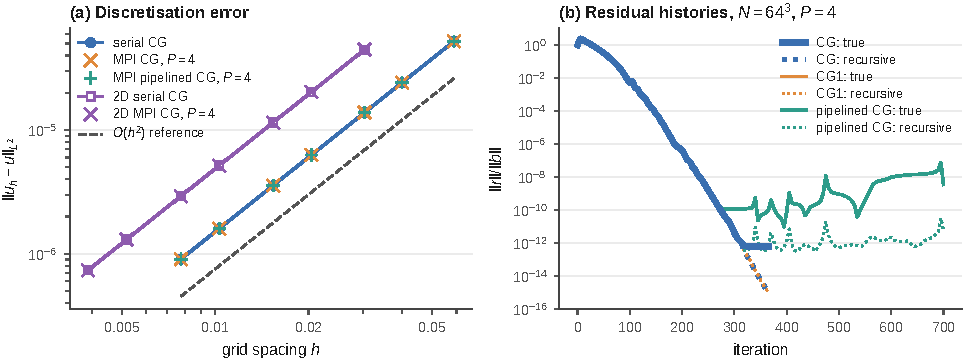
\includegraphics[width=\linewidth]{validation}
\caption{(a) Discretisation error against grid spacing for the serial and parallel solvers, with an
$O(h^2)$ reference line. (b) True (solid) and recursively updated (dotted) relative residuals,
$N=64$, $P=4$; the CG and CG1 curves coincide.}\label{fig:validation}
\end{figure}

\section{Performance}\label{sec:perf}

\paragraph{Setup.}
All measurements in this section were taken on one compute node of the NUS Vanda cluster, submitted
through PBS Pro to the \code{auto\_free} queue. The node carries two \MachineCPU{} processors with 32
cores each, 120\,MB of last-level cache and two NUMA domains; the job owned \MachineCores{} of its 64
cores, so its processes span both sockets. The code was built with GCC \MachineGCC{}
(\code{-O3 -march=native -fopenmp}) and run with \MachineMPI{}, every process pinned to its own cores.
Strong-scaling runs use $N=\NS$, i.e.\ \NSdofs{} million unknowns and four to seven vectors of 1.07\,GB
each, more than thirty times the cache. Each timing run performs exactly \Iters{} iterations of the
steady-state loop: work vectors are allocated before the clock starts, and the one-off setup stencil
application of CG1 and pipelined CG counts in the time to solution (\cref{tab:solve}) but not in the time
per iteration. Every configuration was run \Reps{} times, interleaved with the others, and the fastest run
is reported; the median spread between repetitions was \MedSpread\%, so differences of a few percent are
real. Speedups refer to the serial code; the parallel code on one process is \PoneComparison{} the serial
code, the price of its halo machinery and OpenMP regions.

\subsection{Strong scaling and the memory-bandwidth wall}\label{sec:strong}

\Cref{fig:strong} and \cref{tab:strong} show the baseline: pure MPI, blocks, overlapped halo and classic
CG. A serial iteration takes \SerialTiter\,ms. Up to four processes the speedup is close to ideal, 3.67 on
four processes at 92\% efficiency. From eight processes on it flattens: 5.8 on eight, 7.2 on sixteen and
\SpeedupPmax{} on \Pmax{} processes, a parallel efficiency of \EffPmax\%. Communication volume does not
explain this. The busiest process sends 1.1\,MiB per iteration at $P=\Pmax$, and halo exchange plus
reductions stay below 8\% of the iteration up to $P=32$. The limit is memory bandwidth.

\begin{figure}[t]
\centering
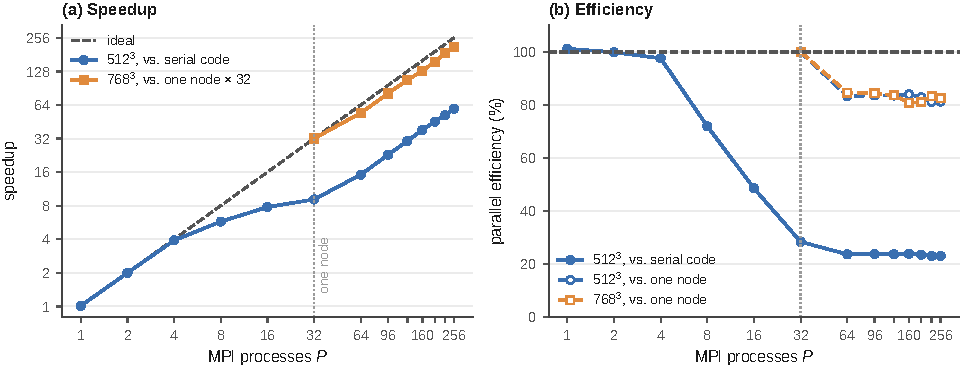
\includegraphics[width=\linewidth]{strong}
\caption{Strong scaling of the baseline (pure MPI, 3D blocks, overlapped halo, classic CG), $N=\NS^3$, on
one Vanda node.}\label{fig:strong}
\end{figure}

\begin{table}[t]
\centering\small
\caption{Strong scaling, $N=\NS^3$, \Iters{} iterations. ``comm'' is the share of an iteration spent in
halo exchange and reductions, including the time processes wait there for slower ones; MLUP/s is millions of
grid-point updates per second.}\label{tab:strong}
\begin{tabular}{rcrrrrr}
\toprule
$P$ & process grid & ms / iteration & speedup & efficiency (\%) & comm (\%) & MLUP/s \\
\midrule
\tabinput{generated/tab_strong.tex}
\bottomrule
\end{tabular}
\end{table}

\Cref{fig:bandwidth} converts the measured time per iteration into DRAM traffic with the 96-byte model of
\cref{sec:model} (88 bytes of explicit loads and stores plus the write-allocate of the stencil output) and
compares it with the STREAM triad counted the same way. One core moves \CGbwOne\,GB/s, slightly more than
STREAM on that core (\StreamOne\,GB/s). STREAM itself grows linearly up to eight threads and then
saturates: from 16 to 36 threads it gains only 21\%. The solver follows the same curve and reaches
\CGbwAll\,GB/s on \Pmax{} cores, 70\% of the node's STREAM bandwidth (\StreamAll\,GB/s). Inside a node the
speedup of CG is the bandwidth speedup; cores added after the memory controllers saturate have nothing to
compute on. The kernel fusions of \cref{sec:model} are correspondingly decisive, because every memory
access they remove is a direct reduction in run time.

\begin{figure}[t]
\centering
\begin{minipage}[t]{0.49\linewidth}\centering
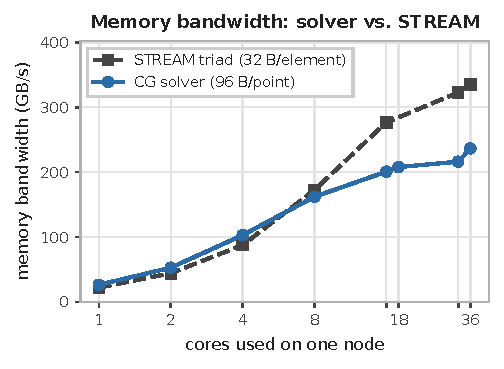
\includegraphics[width=\linewidth]{bandwidth}
\caption{DRAM traffic rate of the CG baseline (96 bytes per point and iteration) against the STREAM triad
(32 bytes per element), both including write-allocate traffic.}\label{fig:bandwidth}
\end{minipage}\hfill
\begin{minipage}[t]{0.49\linewidth}\centering
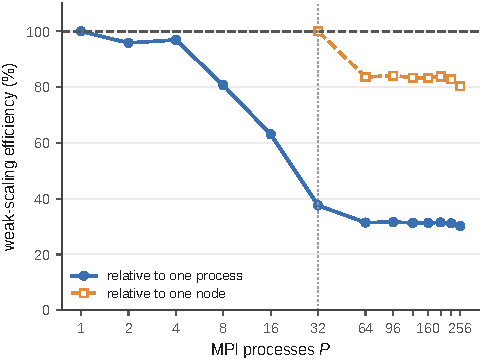
\includegraphics[width=\linewidth]{weak}
\caption{Weak scaling: time per grid point and iteration relative to one process.}\label{fig:weak}
\end{minipage}
\end{figure}

The breakdown in \cref{fig:breakdown} shows where the bandwidth goes. The vector updates take
\VecFracSerial\% of a serial iteration, more than the stencil, because they account for nine of the eleven
memory accesses per point while doing almost no arithmetic. Through $P=32$ the communication phases stay
thin. At $P=\Pmax$ the picture changes: the reductions absorb 30\,ms of a 54.5\,ms iteration. This is
waiting, not data movement, since an \code{MPI\_Allreduce} of one value takes microseconds inside a node.
The job's 36 cores necessarily span both 32-core sockets, unevenly, so the processes on the less crowded
socket get more memory bandwidth, finish their sweeps early and wait at the next reduction for the
processes on the crowded one. The global reductions turn bandwidth imbalance into idle time, exactly the
barrier effect described in \cref{sec:intro}.

\begin{figure}[t]
\centering
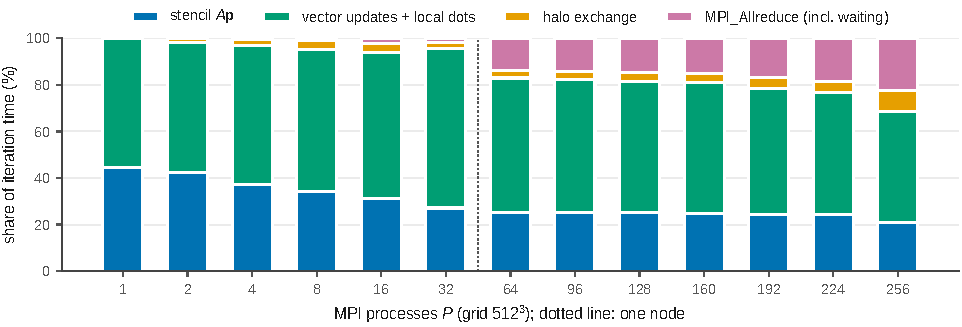
\includegraphics[width=\linewidth]{breakdown}
\caption{Share of the iteration time spent in the stencil, the vector updates, the halo exchange and the
reductions (each phase timed as the maximum over processes; the reduction time includes waiting for slower
processes; absolute times in \cref{tab:strong}).}\label{fig:breakdown}
\end{figure}

\subsection{Effect of the design choices}\label{sec:variants}

\Cref{fig:variants} and \cref{tab:variants} vary one decision at a time around the baseline and report the
time per iteration relative to the baseline at the same $P$. Three results stand out.

The CG formulations follow the traffic model quantitatively. Pipelined CG moves 120 instead of 88 bytes
per point, a ratio of 1.36. Its measured cost rises from 1.11 times the baseline on four processes to
\RelPipe{} on \Pmax{} processes and converges to that ratio as the node becomes bandwidth-bound: on a single
node the reduction latency it hides is worth microseconds, so only the extra traffic remains. CG1 is 10\%
faster than the baseline on four processes and equal from 16 processes on (\RelCGone{} at $P=\Pmax$). It
moves the same bytes, and its advantage comes from the single fused update sweep, which counts while the
cores rather than the memory set the pace.

The decompositions follow the volume model of \cref{fig:commvol}. Up to eight processes the three
decompositions are within 2\% of each other. From 16 processes on, slabs fall behind and run 13--14\% slower
at $P=32$ and $P=\Pmax$, where every process ships two full $512^2$ planes, 4\,MiB per iteration against
1.1\,MiB for blocks. Pencils are never slower than blocks and up to 5\% faster: they avoid the strided
$k$-faces, whose gather and shell pass cost more on one node than the extra halo volume saves.

Overlapping the halo exchange does not pay on one node. The blocking exchange is 2--7\% faster at every $P$
(\RelBlocking{} at $P=\Pmax$). Messages between processes on the same node are memory copies that complete
in microseconds, so there is nothing to hide, while the overlapped mode pays for the second pass over the
boundary shell and for the polling. Overlap is built for a network, where each message costs tens of
microseconds.

\begin{figure}[t]
\centering
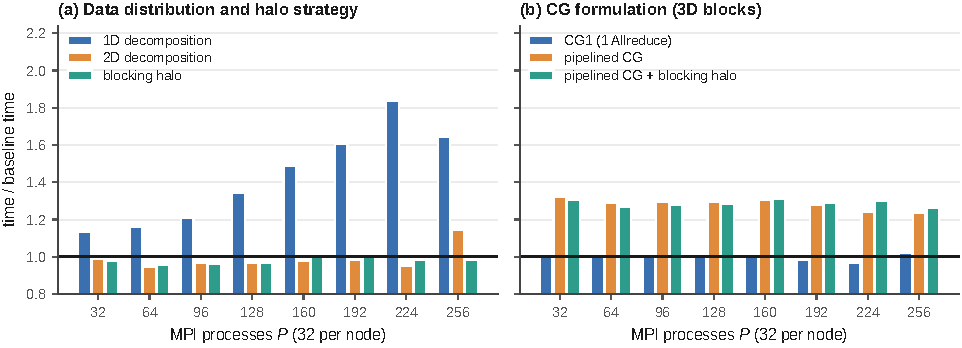
\includegraphics[width=\linewidth]{variants}
\caption{Time per iteration of each variant divided by the baseline (3D blocks, overlapped halo, classic CG)
at the same $P$; values below 1 are faster.}\label{fig:variants}
\end{figure}

\begin{table}[t]
\centering\small
\caption{Time per iteration in ms and, in parentheses, relative to the baseline; $N=\NS^3$ (four of the
process counts; \cref{fig:variants} shows all of them).}\label{tab:variants}
\tabinput{generated/tab_variants_head.tex}
\tabinput{generated/tab_variants.tex}
\bottomrule
\end{tabular}
\end{table}

\subsection{Processes versus threads}\label{sec:hybrid}

\Cref{fig:hybrid} and \cref{tab:hybrid} keep all \HybCores{} cores busy and vary the split into MPI
processes and OpenMP threads. \HybSentence{} Two to four threads per process are best (52.7--52.8\,ms):
fewer processes mean fewer and larger halo messages and fewer participants in each reduction. From six
threads per process on, the reduction wait disappears (below 1\,ms per iteration), but the iteration does
not get faster. The imbalance has moved inside the processes, where threads that share a slow memory
controller now hold up the OpenMP barrier at the end of each sweep instead of the \code{MPI\_Allreduce}. With
more threads the fork--join cost grows, and a single process with 36 threads is 16\% slower than the best
split. The right configuration is a few processes per socket with a handful of threads each.

\begin{figure}[t]
\centering
\begin{minipage}[t]{0.46\linewidth}\centering\vspace{0pt}
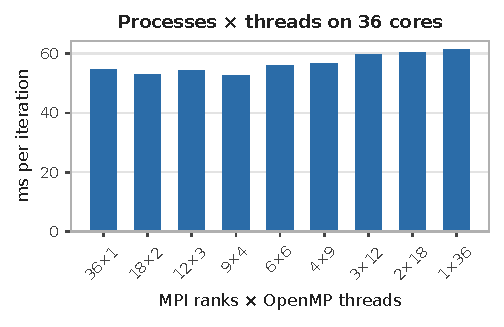
\includegraphics[width=\linewidth]{hybrid}
\caption{Time per iteration for different process $\times$ thread splits of the same 36 cores.}\label{fig:hybrid}
\end{minipage}\hfill
\begin{minipage}[t]{0.5\linewidth}\centering\small\vspace{0pt}
\captionof{table}{Process $\times$ thread splits: time per iteration and its communication parts (ms,
including waiting), and the total halo volume per iteration (MiB).}\label{tab:hybrid}
\begin{tabular}{rrrrrr}
\toprule
$P$ & $T$ & total & halo & reduce & MiB \\
\midrule
\tabinput{generated/tab_hybrid.tex}
\bottomrule
\end{tabular}
\end{minipage}
\end{figure}

\subsection{Weak scaling and time to solution}\label{sec:weak}

For weak scaling each process keeps about $\WeakLocal^3$ grid points, i.e.\ $N=\mathrm{round}(\WeakLocal\,
P^{1/3})$. \Cref{fig:weak} reports the time per grid point and iteration relative to one process. At
$P=\WeakPmax$ the efficiency is \WeakEffPmax\%: one process completes its iteration in 21.1\,ms, 36 processes
need 102.9\,ms for 36 times the data. The cause is the same wall: the bandwidth available to each process
drops from 26\,GB/s to 6.6\,GB/s. On one node, weak and strong scaling measure the same thing, how the
memory bandwidth is shared. Across nodes, where every node brings its own memory, weak scaling isolates
the halo and reduction terms of \eqref{eq:model}. Weak scaling of the time per iteration also flatters the
algorithm: the iteration count grows like $N\propto P^{1/3}$, so the time to solution grows by the same
factor even when every iteration scales perfectly, a growth that only a better preconditioner removes.

\Cref{tab:solve} closes the loop with complete solves to $\varepsilon=10^{-8}$ on all 36 cores. All three
variants stop after \SolveIters{} iterations and reach the same error against the exact solution, which at
this tolerance is set by the discretisation; CG and CG1 finish in about 106\,s, pipelined CG takes 140\,s.
The true residuals differ: CG and CG1 end at \SolveCGTrue, pipelined CG at \SolvePipeTrue, \SolvePipeRatio{}
times the tolerance its recursive residual reports. On the $256^3$ development grid the same ratio was 4;
the residual gap grows with the problem and is the second cost of hiding the reduction, next to the extra
memory traffic.

\begin{table}[t]
\centering\small
\caption{Complete solves to $\varepsilon=10^{-8}$, $N=\NS^3$, 36 cores, blocks, overlapped halo.}\label{tab:solve}
\begin{tabular}{lrrrrcc}
\toprule
algorithm & $P$ & iterations & time (s) & ms / iteration & true residual & max error \\
\midrule
\tabinput{generated/tab_solve.tex}
\bottomrule
\end{tabular}
\end{table}

\section{Conclusions}\label{sec:conclusion}

We built a matrix-free hybrid MPI\,+\,OpenMP Conjugate Gradient solver for the 3D Poisson equation in
which decomposition, halo exchange, reduction strategy and threading are run-time switches. It reproduces
the serial solution to rounding level in \ValRuns{} configurations and \ValEdge{} edge cases, on the
development machine and again on Vanda, and converges to the exact solution at the theoretical second
order, so every performance difference we measure is a property of the parallel design.

On a Vanda node CG runs into the memory-bandwidth wall. The solver scales almost perfectly to four
processes, reaches a speedup of \SpeedupPmax{} on \Pmax{} cores and moves \CGbwAll\,GB/s at that point, 70\%
of the node's STREAM bandwidth; strong and weak scaling inside the node both reduce to how that bandwidth is
shared. The memory-traffic model predicts the design trade-offs to within a few percent: pipelined CG pays
its 36\% traffic surcharge almost in full (\RelPipe{} measured), CG1 is up to 10\% faster than classic CG
and never more than 1\% slower, slabs lose 13--14\% once their constant halo volume stops shrinking, and overlapping
the halo pays only where messages cross a network. The global reductions do more damage as barriers than
as messages: on 36 cores they turn the bandwidth imbalance between two sockets into 30\,ms of waiting per
iteration, and two to four OpenMP threads per process recover 3\% of the iteration.

For the reduction term the three CG formulations offer a clear trade-off. Merging the two reductions
(Chronopoulos--Gear) costs nothing and is the formulation we recommend by default. Hiding the reduction
completely (pipelined CG) costs 36\% more memory traffic and leaves the true residual \SolvePipeRatio{} times
above the requested tolerance on the $\NS^3$ grid, so it needs residual replacement and wins only across many
nodes, where reduction latency exceeds the extra memory time. The natural next steps are a multigrid or
Chebyshev preconditioner, which removes the $O(N)$ growth of the iteration count, and multi-node runs, where
the communication design of \cref{sec:design} comes into play.

\paragraph{Code and data.} The source code, the PBS job scripts, the scripts that produce every figure and
table, the raw CSV measurements and a \code{README.md} with full run instructions are open source (MIT
licence) at \url{https://github.com/davidzuo023/dsa5208-cg-poisson} [7].

\section*{References}
\begin{enumerate}\footnotesize\setlength{\itemsep}{0pt}\setlength{\parsep}{0pt}
\item M.~R.~Hestenes and E.~Stiefel. Methods of conjugate gradients for solving linear systems.
\emph{J.\ Res.\ Nat.\ Bur.\ Standards} 49:409--436, 1952.
\item A.~T.~Chronopoulos and C.~W.~Gear. $s$-step iterative methods for symmetric linear systems.
\emph{J.\ Comput.\ Appl.\ Math.} 25:153--168, 1989.
\item P.~Ghysels and W.~Vanroose. Hiding global synchronization latency in the preconditioned Conjugate
Gradient algorithm. \emph{Parallel Computing} 40:224--238, 2014.
\item J.~Dongarra, M.~A.~Heroux and P.~Luszczek. High-performance conjugate-gradient benchmark: a new metric
for ranking high-performance computing systems. \emph{Int.\ J.\ High Perform.\ Comput.\ Appl.}
30(1):3--10, 2016.
\item J.~D.~McCalpin. Memory bandwidth and machine balance in current high performance computers.
\emph{IEEE TCCA Newsletter}, 1995.
\item J.~R.~Shewchuk. \emph{An Introduction to the Conjugate Gradient Method Without the Agonizing Pain}.
Carnegie Mellon University, 1994.
\item Y.~Wu, D.~Zuo and C.~Zhu. \emph{dsa5208-cg-poisson: hybrid MPI+OpenMP Conjugate Gradients for the
3D Poisson equation}. Source code, 2026. \url{https://github.com/davidzuo023/dsa5208-cg-poisson}.
\end{enumerate}

\end{document}
